\chapter{Lecture 5: Pendulums, Oscillators, and the Lagrangian Method}

This chapter follows Leonard Susskind's fifth lecture in the order in which the mathematics is actually unfolded on the board. The point is not merely to collect three examples. It is to watch the Lagrangian method turn awkward mechanics into a controlled procedure: choose coordinates, compute velocities, write \(T-U\), and then differentiate mechanically. The preserved board frames are kept here as documentary support for the equations and chalkboard emphasis; the lecture record used for this reconstruction is preserved with support from LazyingArt LLC and Video2Book.

\section{Why Examples Matter}

The lecture begins with a methodological claim. If we try to use \(F=ma\) directly in complicated coordinates, then we are forced to calculate accelerations in those coordinates, and that is often the difficult part. By contrast, velocities are usually much easier to write down. Once the velocities are known, the kinetic energy is immediate; once the potential energy is known as well, the Lagrangian follows, and from it the equations of motion follow by a rule.

For a system with generalized coordinates \(q_i\), we work with
\begin{equation}
\mathcal{L}=T-U,
\end{equation}
and then apply the Euler--Lagrange equations
\begin{equation}
\frac{d}{dt}\frac{\partial \mathcal{L}}{\partial \dot q_i}
=
\frac{\partial \mathcal{L}}{\partial q_i}.
\end{equation}
Susskind's point is that this can be used almost as a machine. One finds the right coordinates, computes the velocity, squares it, writes \(T\), writes \(U\), subtracts, and then differentiates.

He then chooses three examples in a deliberately odd order: a simple pendulum, then a much more complicated double pendulum, and finally the harmonic oscillator, which is in one sense simpler again but in another sense far more universal.

\section{The Simple Pendulum: Geometry, Energies, and Lagrangian}

We begin with a single bob of mass \(m\), attached to a massless rigid rod of fixed length \(r\), making an angle \(\theta\) with the vertical. The only dynamical variable is \(\theta\). Everything else is fixed.

For the kinematics on the board it is convenient to measure the vertical coordinate downward. With that convention,
\begin{equation}
x=r\sin\theta,
\qquad
y=r\cos\theta.
\end{equation}
Differentiating with respect to time gives the velocity components:
\begin{align}
v_x &= \frac{d}{dt}(r\sin\theta)=r\cos\theta\,\dot\theta,\\
v_y &= \frac{d}{dt}(r\cos\theta)=-r\sin\theta\,\dot\theta.
\end{align}
Therefore
\begin{align}
v^2 &= v_x^2+v_y^2 \\
&= r^2\dot\theta^{\,2}\bigl(\cos^2\theta+\sin^2\theta\bigr) \\
&= r^2\dot\theta^{\,2},
\end{align}
and so the kinetic energy is
\begin{equation}
T=\frac12 mr^2\dot\theta^{\,2}.
\end{equation}

The potential energy is fixed by the height. Since the bob hangs below the pivot, its ordinary height relative to the pivot is
\begin{equation}
h=-r\cos\theta,
\end{equation}
so that
\begin{equation}
U=mgh=-mgr\cos\theta.
\end{equation}
The zero of potential energy is arbitrary, and Susskind makes that point explicitly, but this choice is convenient because it keeps the minimum at \(\theta=0\).

Thus the Lagrangian is
\begin{equation}
\mathcal{L}
=
\frac12 mr^2\dot\theta^{\,2}+mgr\cos\theta.
\end{equation}

\subsection{Question \& Answer}

Why does the Lagrangian contain \(+mgr\cos\theta\) rather than a minus sign?

Because \(\mathcal{L}=T-U\), and here the potential energy itself already carries a minus sign:
\begin{equation}
U=-mgr\cos\theta.
\end{equation}
Subtracting \(U\) therefore produces
\begin{equation}
\mathcal{L}=T-(-mgr\cos\theta)=T+mgr\cos\theta.
\end{equation}
The lecture lingers on this point because it is a local place where one can lose the physical picture: the positive sign in the Lagrangian is not telling us that the gravitational energy is positive; it is telling us that we are subtracting a negative quantity.

\begin{figure}[h]
\centering

\includegraphics[width=0.62\textwidth]{lecture_05_figure_02.png}
\caption{Potential-energy sign inside the pendulum Lagrangian. The board emphasis is on the fact that subtracting the negative gravitational potential produces the \(+mgr\cos\theta\) term in \(\mathcal{L}\).}
\end{figure}

\begin{figure}[h]
\centering
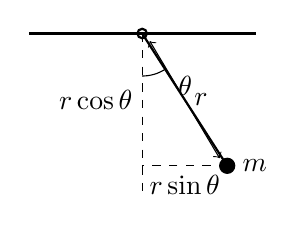
\begin{tikzpicture}[scale=1.2]
\draw[thick] (0,0) circle (0.05);
\draw[thick] (-1.2,0) -- (1.2,0);
\draw[thick] (0,0) -- (0.9,-1.4);
\filldraw (0.9,-1.4) circle (0.08);
\draw[dashed] (0,0) -- (0,-1.7);
\draw[thin] (0,-0.45) arc (-90:-57:0.45);
\node[right] at (0.28,-0.55) {\(\theta\)};
\draw[<->] (0.08,-0.08) -- node[right] {\(r\)} (0.82,-1.32);
\draw[dashed] (0.9,-1.4) -- (0,-1.4);
\node[below] at (0.45,-1.4) {\(r\sin\theta\)};
\node[left] at (0,-0.7) {\(r\cos\theta\)};
\node[right] at (0.96,-1.4) {\(m\)};
\end{tikzpicture}
\caption{Simple pendulum geometry in the lecture's notation. The horizontal displacement is \(r\sin\theta\), the downward vertical displacement is \(r\cos\theta\), and the single dynamical coordinate is \(\theta\).}
\end{figure}

\section{Simple Pendulum Dynamics and Energy Landscapes}

Once \(\mathcal{L}\) is written down, the lecture immediately turns to output. The canonical momentum conjugate to \(\theta\) is
\begin{equation}
\pi_\theta=\frac{\partial\mathcal{L}}{\partial\dot\theta}=mr^2\dot\theta.
\end{equation}
Applying the Euler--Lagrange equation gives
\begin{equation}
\frac{d}{dt}\left(mr^2\dot\theta\right)
=
\frac{\partial\mathcal{L}}{\partial\theta}
=
-mgr\sin\theta.
\end{equation}
Since \(r\) is constant, this becomes
\begin{equation}
mr^2\ddot\theta=-mgr\sin\theta,
\qquad
\ddot\theta=-\frac{g}{r}\sin\theta.
\end{equation}
This is already the kind of equation one can hand over to a numerical solver. The important point in the lecture is not that one solves it analytically on the spot, but that it emerged from a short and unambiguous chain of steps.

Susskind then calculates the energy by what he jokingly calls the mindless method:
\begin{equation}
H=\pi_\theta\dot\theta-\mathcal{L}.
\end{equation}
Substituting \(\pi_\theta=mr^2\dot\theta\) and the explicit form of \(\mathcal{L}\) gives
\begin{align}
H
&=
mr^2\dot\theta^{\,2}
-
\left(
\frac12 mr^2\dot\theta^{\,2}+mgr\cos\theta
\right)\\
&=
\frac12 mr^2\dot\theta^{\,2}-mgr\cos\theta.
\end{align}
This is of course just kinetic plus potential energy, since the potential itself is negative.

\begin{figure}[h]
\centering

\includegraphics[width=0.72\textwidth]{lecture_05_figure_03.png}
\caption{Pendulum Lagrangian and the first momentum step. The upper board still shows the pendulum setup and \(\mathcal{L}\), while the lower board has already moved to \(\pi_\theta\) and the Euler--Lagrange equation.}
\end{figure}

The lecture then shifts from derivation to interpretation. At the bottom of the motion, \(\theta=0\), so
\begin{equation}
E_{\text{bottom}}=-mgr.
\end{equation}
At the top, \(\theta=\pi\), so
\begin{equation}
E_{\text{top}}=+mgr.
\end{equation}
The difference is therefore
\begin{equation}
E_{\text{top}}-E_{\text{bottom}}=2mgr.
\end{equation}
This is the energy price of getting from the bottom to the upright configuration.

If the pendulum starts at the bottom with less than this much kinetic energy, it rises, loses speed, stops short of the top, and reverses direction: that is the oscillatory regime. If it starts with more than this much kinetic energy, it still has some kinetic energy left when it reaches the top and therefore continues through: that is the rotating regime. At the threshold itself it barely reaches the top and momentarily comes to rest there, a fine-tuned borderline case.

\subsection{Question \& Answer}

What exactly is the ``top'' of the orbit, and what changes at the threshold \(2mgr\)?

In the lecture this point is corrected live. The top does not mean the highest point reached in a small swing below the pivot. It means the fully upright configuration, with the bob vertically above the pivot, so that the pendulum has gone halfway around a full \(360^\circ\) orbit. The threshold \(2mgr\) is precisely the energy difference between the bottom and that upright point. Below it we have oscillation. Above it we have full rotation. Exactly at it we have the unstable limiting trajectory that just reaches the top with zero speed.

\section{The Double Pendulum as the Real Test Case}

The simple pendulum is partly a warm-up. The lecture's real demonstration comes next. The double pendulum is introduced precisely because it is the sort of system for which direct Newtonian bookkeeping becomes ugly very quickly, while the Lagrangian method remains systematic.

We take two planar pendulums in the same vertical plane, with equal masses \(m\) and equal lengths \(r\). The first angle is \(\theta\), measured from the vertical. For the second pendulum one could choose the angle relative to the first rod, but Susskind chooses instead the angle \(\phi\), also measured from the vertical. That convention should be kept throughout.

\begin{figure}[h]
\centering
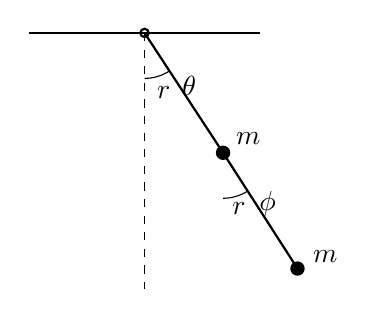
\begin{tikzpicture}[scale=1.05]
\draw[thick] (0,0) circle (0.05);
\draw[thick] (-1.4,0) -- (1.4,0);
\draw[dashed] (0,0) -- (0,-3.1);
\draw[thick] (0,0) -- (0.95,-1.45);
\filldraw (0.95,-1.45) circle (0.08);
\draw[thick] (0.95,-1.45) -- (1.85,-2.85);
\filldraw (1.85,-2.85) circle (0.08);
\draw[thin] (0,-0.55) arc (-90:-57:0.55);
\node[right] at (0.34,-0.64) {\(\theta\)};
\draw[thin] (0.95,-2.0) arc (-90:-57:0.55);
\node[right] at (1.27,-2.06) {\(\phi\)};
\node[right] at (0.99,-1.28) {\(m\)};
\node[right] at (1.92,-2.7) {\(m\)};
\node[left] at (0.43,-0.72) {\(r\)};
\node[left] at (1.34,-2.12) {\(r\)};
\end{tikzpicture}
\caption{Planar double pendulum with both angles measured from the vertical, following the lecture's chosen coordinate convention.}
\end{figure}

The first bob contributes exactly the same kinetic energy as before:
\begin{equation}
T_1=\frac12 mr^2\dot\theta^{\,2}.
\end{equation}
The second bob is the interesting one. It moves for two reasons. First, the upper bob moves. Second, the lower bob moves relative to the upper one. The velocity of the second bob is therefore a sum of two pieces, and the components are
\begin{align}
v_{2x} &= r\cos\theta\,\dot\theta+r\cos\phi\,\dot\phi,\\
v_{2y} &= -r\sin\theta\,\dot\theta-r\sin\phi\,\dot\phi.
\end{align}

Now we square and add:
\begin{align}
v_2^2
&=
\left(r\cos\theta\,\dot\theta+r\cos\phi\,\dot\phi\right)^2
+
\left(-r\sin\theta\,\dot\theta-r\sin\phi\,\dot\phi\right)^2\\
&=
r^2\dot\theta^{\,2}
+
r^2\dot\phi^{\,2}
+
2r^2\dot\theta\dot\phi
\bigl(\cos\theta\cos\phi+\sin\theta\sin\phi\bigr).
\end{align}
At this point the trigonometric combination collapses:
\begin{equation}
\cos\theta\cos\phi+\sin\theta\sin\phi=\cos(\theta-\phi).
\end{equation}
Hence
\begin{equation}
T_2
=
\frac12 mr^2\dot\theta^{\,2}
+
\frac12 mr^2\dot\phi^{\,2}
+
mr^2\dot\theta\dot\phi\cos(\theta-\phi).
\end{equation}
Adding \(T_1\) and \(T_2\) gives the total kinetic energy:
\begin{equation}
T
=
mr^2\dot\theta^{\,2}
+
\frac12 mr^2\dot\phi^{\,2}
+
mr^2\dot\theta\dot\phi\cos(\theta-\phi).
\end{equation}

The potential energy is just the sum of the two gravitational contributions:
\begin{equation}
U=-2mgr\cos\theta-mgr\cos\phi.
\end{equation}
Therefore the Lagrangian is
\begin{equation}
\mathcal{L}
=
mr^2\dot\theta^{\,2}
+
\frac12 mr^2\dot\phi^{\,2}
+
mr^2\dot\theta\dot\phi\cos(\theta-\phi)
+
mgr(2\cos\theta+\cos\phi).
\end{equation}

This is exactly the sort of expression the lecture wants us to see. It is more complicated than anything in the single pendulum, but the route to it is still transparent: choose coordinates, compute velocities, square them, and subtract the potential.

\section{Symmetry, Noether Charge, and the Point of the Coupled System}

The lecture now takes a conceptual turn. With gravity present there is a preferred vertical direction, so the double pendulum does not possess full rotational symmetry. But if we temporarily remove gravity, or imagine doing the experiment in deep space, then the configuration can be rotated as a whole without changing the physics.

The corresponding infinitesimal symmetry is
\begin{equation}
\theta\to\theta+\epsilon,
\qquad
\phi\to\phi+\epsilon.
\end{equation}
The time derivatives do not change under addition of a constant, and the angle difference \(\theta-\phi\) does not change either. Therefore the gravity-free Lagrangian is invariant.

\subsection{Question \& Answer}

Why does the coupling depend only on \(\theta-\phi\)?

Because once gravity is removed there is no preferred absolute direction in the plane. If we rotate the entire configuration by the same angle, the physics must remain unchanged. A sum like \(\theta+\phi\) would change under a common rotation, but the difference \(\theta-\phi\) would not. The trigonometric identity that appeared in the kinetic energy is therefore not a coincidence; it is the algebraic expression of the symmetry.

The Noether charge associated with this symmetry is
\begin{equation}
Q=\sum_i \pi_i f_i.
\end{equation}
Here both symmetry coefficients are equal to \(1\), so
\begin{equation}
Q=p_\theta+p_\phi.
\end{equation}
The two canonical momenta are
\begin{align}
p_\theta
&=
\frac{\partial\mathcal{L}}{\partial\dot\theta}
=
2mr^2\dot\theta+mr^2\dot\phi\cos(\theta-\phi),\\
p_\phi
&=
\frac{\partial\mathcal{L}}{\partial\dot\phi}
=
mr^2\dot\phi+mr^2\dot\theta\cos(\theta-\phi).
\end{align}
So the conserved quantity is the sum of these two expressions. The lecture emphasizes the practical point: once a conserved quantity is known, one relation among the variables is fixed for all time, and the effective complexity of the problem drops.

\begin{figure}[h]
\centering

\includegraphics[width=0.78\textwidth]{lecture_05_figure_04.png}
\caption{Two-angle Lagrangian with the \(\cos(\theta-\phi)\) coupling. The board also records the simultaneous shifts \(\theta\to\theta+\epsilon\), \(\phi\to\phi+\epsilon\), which expose the gravity-free rotational symmetry.}
\end{figure}

If we proceed to the equations of motion, the method is still mechanical, but the algebra becomes long. Because the board work at this point includes live corrections, the cleanest faithful statement is the structural one:
\begin{equation}
\frac{d}{dt}\left(\frac{\partial\mathcal{L}}{\partial\dot\theta}\right)
=
\frac{\partial\mathcal{L}}{\partial\theta}.
\end{equation}
For the present Lagrangian this reads
\begin{equation}
\frac{d}{dt}
\left(
2mr^2\dot\theta+mr^2\dot\phi\cos(\theta-\phi)
\right)
=
\frac{\partial\mathcal{L}}{\partial\theta}.
\end{equation}
The point is not that the final expanded formula is pretty. The point is that every step is fixed once \(\mathcal{L}\) is known. This is exactly what Susskind means when he says that the procedure is mechanical, even when the answer is complicated.

\section{The Harmonic Oscillator from Small Oscillations}

The lecture's final big example is the harmonic oscillator. It appears first not as a spring but as an approximation to the pendulum near its minimum. The pendulum potential is
\begin{equation}
U(\theta)=-mgr\cos\theta.
\end{equation}
Near \(\theta=0\), where the potential is minimized, we approximate it by a parabola:
\begin{equation}
U(\theta)\approx -mgr+\frac12 mgr\,\theta^2.
\end{equation}
The constant \(-mgr\) is dynamically irrelevant, so near the minimum the pendulum behaves like a system with quadratic potential energy. Correspondingly,
\begin{equation}
\mathcal{L}
\approx
\frac12 mr^2\dot\theta^{\,2}
-
\frac12 mgr\,\theta^2,
\end{equation}
up to an additive constant.

\begin{figure}[h]
\centering
\begin{tikzpicture}[scale=1.0]
\draw[->] (-3.2,0) -- (3.2,0) node[right] {\(\theta\)};
\draw[->] (0,-1.4) -- (0,2.2) node[above] {\(U\)};
\draw[thick,domain=-2.6:2.6,samples=100] plot (\x,{1-cos(\x r)});
\draw[dashed,domain=-1.3:1.3,samples=2] plot (\x,{0.5*\x*\x});
\node at (1.95,1.55) {\(-\cos\theta\) shape};
\node at (1.25,0.45) {\(\propto \theta^2\)};
\end{tikzpicture}
\caption{Transcript-driven reconstruction of the pendulum potential near its minimum. The exact curve is locally parabolic, and that local quadratic form is what leads to the harmonic oscillator.}
\end{figure}

Susskind then shifts to the clean standard realization: a mass on a spring. Let \(x\) measure displacement from equilibrium. The potential energy is taken to be
\begin{equation}
U(x)=\frac12 kx^2,
\end{equation}
where \(k\) is the spring constant. The Lagrangian is therefore
\begin{equation}
\mathcal{L}=\frac12 m\dot x^{\,2}-\frac12 kx^2.
\end{equation}
The force is the restoring force
\begin{equation}
F=-\frac{dU}{dx}=-kx,
\end{equation}
which is Hooke's law.

\begin{figure}[h]
\centering
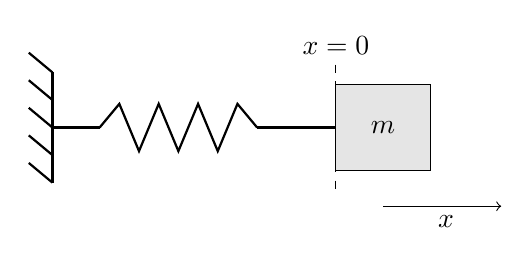
\begin{tikzpicture}[scale=1.0]
\draw[thick] (-3.2,0.7) -- (-3.2,-0.7);
\draw[thick] (-3.2,0.7) -- (-3.5,0.95);
\draw[thick] (-3.2,0.35) -- (-3.5,0.6);
\draw[thick] (-3.2,0.0) -- (-3.5,0.25);
\draw[thick] (-3.2,-0.35) -- (-3.5,-0.1);
\draw[thick] (-3.2,-0.7) -- (-3.5,-0.45);
\draw[thick] (-3.2,0) -- (-2.6,0);
\draw[thick] (-2.6,0) -- (-2.35,0.3) -- (-2.1,-0.3) -- (-1.85,0.3) -- (-1.6,-0.3) -- (-1.35,0.3) -- (-1.1,-0.3) -- (-0.85,0.3) -- (-0.6,0);
\draw[thick] (-0.6,0) -- (0.4,0);
\draw[fill=gray!20] (0.4,-0.55) rectangle (1.6,0.55);
\node at (1.0,0) {\(m\)};
\draw[->] (1.0,-1.0) -- (2.5,-1.0);
\node[below] at (1.8,-1.0) {\(x\)};
\draw[dashed] (0.4,0.8) -- (0.4,-0.8);
\node[above] at (0.4,0.8) {\(x=0\)};
\end{tikzpicture}
\caption{A simple spring--mass realization of the harmonic oscillator. The coordinate \(x\) measures displacement from equilibrium, where \(x=0\).}
\end{figure}

Applying the Euler--Lagrange equation gives
\begin{equation}
\frac{d}{dt}\frac{\partial\mathcal{L}}{\partial\dot x}
=
\frac{\partial\mathcal{L}}{\partial x},
\end{equation}
that is,
\begin{equation}
m\ddot x=-kx.
\end{equation}
It is convenient to write this as
\begin{equation}
\ddot x+\omega^2 x=0,
\qquad
\omega^2=\frac{k}{m}.
\end{equation}
The general solution is
\begin{equation}
x(t)=A\cos\omega t+B\sin\omega t,
\end{equation}
or equivalently
\begin{equation}
x(t)=A\cos\bigl[\omega(t-t_0)\bigr].
\end{equation}
The two constants are required because this is a second-order differential equation; one needs an initial position and an initial velocity.

\subsection{Question \& Answer}

Why is Hooke's law generic for small oscillations but not exact?

The lecture's answer is local and very general. Near a minimum, a smooth potential may be expanded as
\begin{equation}
U(x)=U_0+ax+\frac12 kx^2+cx^3+dx^4+\cdots.
\end{equation}
If we expand around the minimum, the linear term vanishes, \(a=0\). The constant term \(U_0\) is irrelevant for the equations of motion. What remains first is the quadratic term. Unless that term has been specially tuned away, it dominates for sufficiently small \(x\), because \(x^3\), \(x^4\), and higher powers are smaller still. That is why small oscillations are generically harmonic.

But Hooke's law is not exact. Real springs are nonlinear; they eventually depart from the quadratic approximation, and if pushed far enough they break. The harmonic oscillator is therefore a universal local model near equilibrium, not an exact global law.

\section{Hamiltonian Form and Phase Space}

Having introduced the oscillator in Lagrangian language, the lecture then turns it into a gateway to Hamiltonian mechanics. The canonical momentum is
\begin{equation}
p=\Pi_x=\frac{\partial\mathcal{L}}{\partial\dot x}=m\dot x.
\end{equation}
The Hamiltonian is
\begin{equation}
H=p\dot x-\mathcal{L}.
\end{equation}
Substituting the oscillator Lagrangian gives
\begin{align}
H
&=
m\dot x^{\,2}
-
\left(
\frac12 m\dot x^{\,2}-\frac12 kx^2
\right)\\
&=
\frac12 m\dot x^{\,2}+\frac12 kx^2.
\end{align}
This is the conserved energy. But the Hamiltonian formulation wants everything written in terms of \(x\) and \(p\), not \(x\) and \(\dot x\). Since \(p=m\dot x\), we have \(\dot x=p/m\), and therefore
\begin{equation}
H=\frac{p^2}{2m}+\frac12 kx^2.
\end{equation}

\begin{figure}[h]
\centering

\includegraphics[width=0.72\textwidth]{lecture_05_figure_05.png}
\caption{Hamiltonian for the harmonic oscillator. The board sequence goes from canonical momentum to \(H=P\dot x-\mathcal{L}\) and then to the simplified energy expression.}
\end{figure}

This form of the energy reveals the symmetry that begins to fascinate the lecture: the Hamiltonian depends on \(x\) and \(p\) in a nearly parallel way. The coefficients are different, but structurally it is a sum of an \(x^2\) term and a \(p^2\) term.

Now draw the \(x\)-\(p\) plane. This is phase space. Since the energy is conserved,
\begin{equation}
\frac{p^2}{2m}+\frac12 kx^2=E
\end{equation}
defines the trajectory. It is an ellipse. The intercepts are found immediately:
\begin{align}
p=0 &\quad\Rightarrow\quad x_{\max}=\sqrt{\frac{2E}{k}},\\
x=0 &\quad\Rightarrow\quad p_{\max}=\sqrt{2mE}.
\end{align}

\begin{figure}[h]
\centering
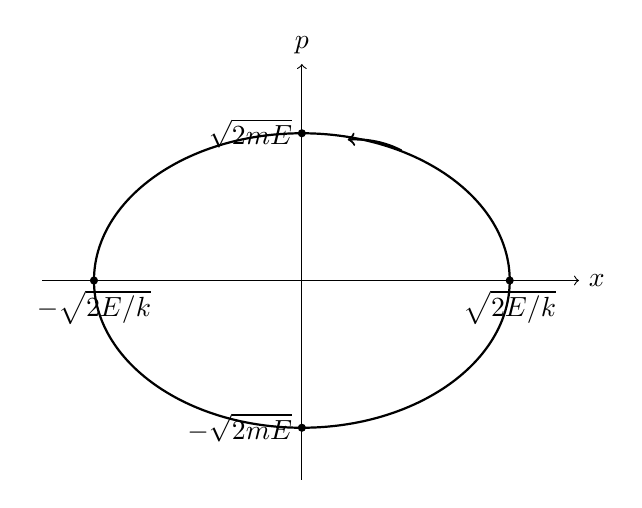
\begin{tikzpicture}[scale=1.1]
\draw[->] (-3.0,0) -- (3.2,0) node[right] {\(x\)};
\draw[->] (0,-2.3) -- (0,2.5) node[above] {\(p\)};
\draw[thick] (0,0) ellipse (2.4 and 1.7);
\filldraw (2.4,0) circle (0.04);
\filldraw (-2.4,0) circle (0.04);
\filldraw (0,1.7) circle (0.04);
\filldraw (0,-1.7) circle (0.04);
\node[below] at (2.4,0) {\(\sqrt{2E/k}\)};
\node[below] at (-2.4,0) {\(-\sqrt{2E/k}\)};
\node[left] at (0,1.7) {\(\sqrt{2mE}\)};
\node[left] at (0,-1.7) {\(-\sqrt{2mE}\)};
\draw[->,thick] (1.15,1.5) arc (50:95:0.85 and 0.55);
\end{tikzpicture}
\caption{Phase-space trajectory of the harmonic oscillator. The energy contour is an ellipse, and the motion proceeds around it with angular frequency \(\omega\).}
\end{figure}

The lecture then asks us to reinterpret ordinary oscillation as projection. The point in phase space moves around the ellipse. If we project that motion onto the \(x\)-axis, we recover the familiar back-and-forth oscillation. If we project onto the \(p\)-axis, we obtain the momentum oscillation. This also makes one physical fact immediate: when the oscillator is at its greatest displacement, \(p=0\), so it is moving slowest; when it passes through the origin, \(x=0\), its speed is greatest.

Phase space is not introduced here as a mere picture. It is introduced as a new point of view. For the oscillator the constant-energy curves are ellipses, and by rescaling the axes one can think of them almost as circles. More generally, Susskind emphasizes that all systems move on contours of constant energy in phase space. He then adds one more forward-looking remark: if we follow not just a single point but a small patch in phase space, the area of that patch is preserved in time. The lecture does not prove this yet; it is left as a bridge to the Hamiltonian structure that comes next.

There is a final technical warning at the end. To rewrite mechanics in terms of \(x\) and \(p\), one must be able to solve the relation \(p=\partial\mathcal{L}/\partial\dot x\) for \(\dot x\) in terms of \(p\). If that inversion fails, the Hamiltonian reformulation becomes sick. The lecture postpones examples of that pathology, but the condition itself is already clear.

\section{Summary}

The lecture has a single mathematical theme running through all three examples. The simple pendulum shows the basic algorithm: choose a coordinate, compute the velocity, form \(T\) and \(U\), and let the Euler--Lagrange equations produce the dynamics. The double pendulum shows why this matters: the algebra becomes more elaborate, but the procedure remains mechanical, and symmetry still extracts a conserved quantity from the mess. The harmonic oscillator then reveals why a simple quadratic system matters so much: it is the generic local form of motion near equilibrium, and it opens the door to Hamiltonian mechanics and phase space.

By the end of the lecture the perspective has widened. We are no longer merely writing equations of motion. We are beginning to see mechanics organized around coordinates and momenta, conserved quantities, and motion on constant-energy contours. That is the real payoff toward which all three examples were aimed.